\section{Excelleren}
\subsection{De PCB}
\subsubsection{Voordeel voor de klant/ gebruiker van ...}
Wij hebben gekozen om een pcb te ontwerpen voor ons circuit omdat een PCB een stuk compacter is en lichter is in vergelijking met een breadboard of een met de hand gesoldeerd circuit, wat bevorderlijk is voor de miniaturisering van elektronische apparatuur. En nog is het bevorderlijk voor gemechaniseerde en geautomatiseerde productie, verbetert de arbeidsproductiviteit en verlaagt de kosten van elektronische apparatuur. Dit zorgt voor goedkopere prijzen voor de consument.  

\subsubsection{Nadelen kosten van ...}
Een mogelijk nadeel van het gebruik van PCB's is de grotere moeilijkheid bij reparatie als er gebruik word gemaakt van SMD-componenten. Een ander nadeel is dat het niet mogelijk is om een doorgekraste lijn op een PCB simpel te repareren. Als laatst is het zo dat een PCB die gebruik maakt van SMD-componenten een stuk duurder is sinds het nodig is om een machine voor elke lay-out in te stellen wat veel tijd en geld kost. Dit is dus niet rendabel bij een kleinere productie. Maar anders dan dat zijn de nadelen bijna niet te vinden onder normale omstandigheden. Een PCB is namelijk niet geschikt voor circuits die gebruik maken van hoge stromen want dat kunnen de materialen niet aan. 



\subsubsection{Hoe werkt ... en hoe ziet ... er uit}
Een PCB werkt als volgt: je creëert een schema van het circuit met alle componenten en waardes. Hiermee design je pcb-design waarop je alle componenten een locatie geeft en daartussen koperen lijnen trekt die je dan laat produceren. De PCB werkt dan ook niet anders dan een circuit op een breadboard. In dit geval stellen de koperen lijnen tussen de componenten de bedrading op het breadboard voor. Doordat de bedrading zich in de PCB bevindt is er een betere connectie tussen de componenten.  Bij PCB's is er ook de mogelijkheid om SMD-componenten te gebruiken. Dit zijn miniatuurversies van standaard componenten die een stuk minder ruimte en materiaal opnemen. Wijzelf hebben gekozen voor THT-onderdelen. THT betekent dat er wat gaten in de PCB zitten voor standaard componenten wat handig is wanneer componenten makkelijk te vervangen moeten zijn.

\newpage
In figuur 5 zie je een 3d render van onze PCB. Zoals je kan zien zijn er een heleboel gaten met uitlijnen van componenten. Dit zijn footprints voor THT-componenten oftewel standaard componenten. Op de PCB zitten ook wat plaatsen voor externe connecties zoals de voeding en speaker aan de rechterkant. In de hoeken hebben wij ook wat bevestigingsgaten voor schroeven. Deze gaten zijn verbonden aan grond. Als er goed gekeken wordt vallen er ook wat uitgezonderde lijnen te zien. Dit is de bedrading van de PCB tussen de componenten. Voor grond en positief hebben wij geen lijnen getrokken maar de standaard manier gebruikt waar een hele zijde wordt toegekend aan grond en de ander aan positief. 
 
\begin{figure}[ht]
    \centering
    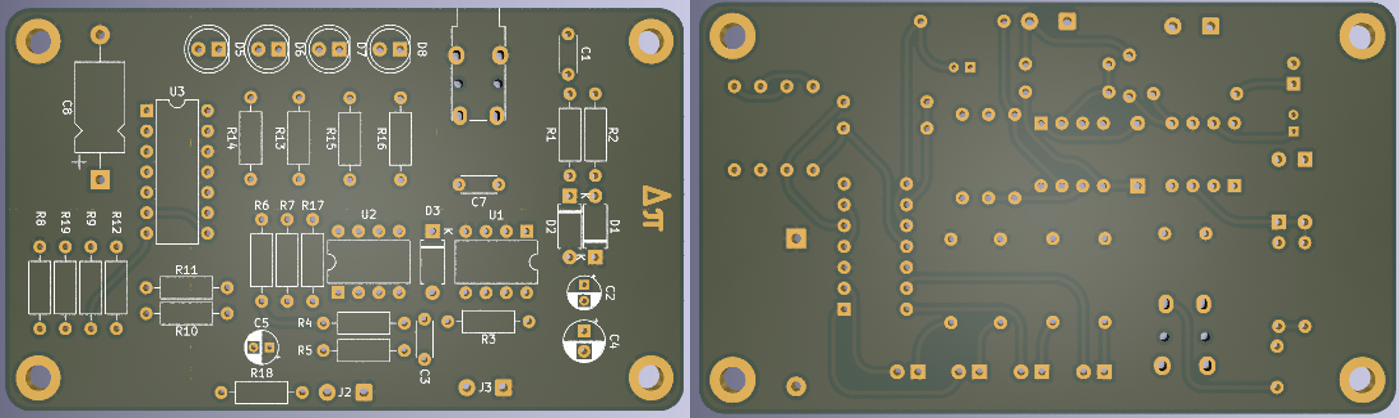
\includegraphics[width=0.90\textwidth]{IMG/004/PCB.png}
    \caption{PCB}
    \label{fig:PCB}
\end{figure}